\section{Results}

\subsection{Data Summary and Model Selection}

In total, we analyzed 1,894 observation pairs spanning 115 unique deployment–day combinations. We evaluated 47 candidate models within a generalized additive mixed modeling (GAMM) framework and performed model selection using Akaike's Information Criterion (AIC).

The best-supported model included smooth terms for average temperature, direct sun exposure, time within day, and the lagged butterfly count. This best-fit model (label: \texttt{M22\_temp\_time}) had an AIC of 8081.848, a \(\Delta\)AIC of 0.0, and an AIC weight of 0.88, indicating it received 88\% of the support among all candidates. The next-best model (\texttt{M21\_time\_of\_day}) was 4.796 AIC units higher (AIC = 8086.644), reflecting substantially weaker support.

% Model selection table (top 10)
\begin{table}

\caption{\label{tab:export-model-selection-table}Top 5 candidate models ranked by AIC for monarch butterfly abundance change analysis. All terms are smooth unless marked as (linear). Wind p-value shows significance of max_gust term when present in model.}
\centering
\begin{tabular}[t]{llrrrrl}
\toprule
Model ID & Model Terms & AIC & <U+0394>AIC & AIC Weight & df & Wind p-value\\
\midrule
M50 & \textbullet\ Previous butterfly count\\ \textbullet\ Temperature\\ \textbullet\ Time since sunrise\\ \textbullet\ ti(Maximum wind speed, Butterflies in direct sun) & 8078.029 & 0.000 & 0.8559 & 15 & 5.55e-05\\
M23 & \textbullet\ Previous butterfly count\\ \textbullet\ Temperature\\ \textbullet\ Butterflies in direct sun\\ \textbullet\ Time since sunrise & 8081.848 & 3.820 & 0.1268 & 14 & NA\\
M22 & \textbullet\ Previous butterfly count\\ \textbullet\ Temperature (linear)\\ \textbullet\ Butterflies in direct sun\\ \textbullet\ Time since sunrise & 8086.644 & 8.615 & 0.0115 & 13 & NA\\
M24 & \textbullet\ Previous butterfly count\\ \textbullet\ Maximum wind speed\\ \textbullet\ Temperature\\ \textbullet\ Butterflies in direct sun\\ \textbullet\ Time since sunrise & 8088.049 & 10.020 & 0.0057 & 16 & 0.218\\
M52 & \textbullet\ Temperature\\ \textbullet\ Time since sunrise\\ \textbullet\ ti(Maximum wind speed, Butterflies in direct sun) & 8096.722 & 18.693 & 0.0001 & 13 & 1.13e-05\\
\bottomrule
\end{tabular}
\end{table}


\subsection{Best-Fit Model Structure and Effects}

The best-fit model had the form:
\begin{quote}
\texttt{butterfly\_difference\_cbrt \textasciitilde\ s(total\_butterflies\_t\_lag) + s(temperature\_avg) + s(butterflies\_direct\_sun\_t\_lag) + s(time\_within\_day\_t)}
\end{quote}

This model explained a modest portion of the variability (adjusted \(R^2\) = 0.0568) but identified several statistically and biologically meaningful patterns:

- Lagged roost size, \(s(\texttt{total\_butterflies\_t\_lag})\): A significant, non-linear negative association with subsequent change in abundance (edf = 2.621, \(F\) = 12.020, \(p = 8.26 \times 10^{-7}\)). Larger initial roosts tended to decline more in the next interval (see Figure~\ref{fig:partial_effects}).
- Average temperature, \(s(\texttt{temperature\_avg})\): A significant, non-linear relationship (edf = 3.930, \(F\) = 3.230, \(p = 0.0283\)), with the effect peaking near \(\sim\!20\,^{\circ}\mathrm{C}\) before declining (Figure~\ref{fig:partial_effects}).
- Direct sun exposure, \(s(\texttt{butterflies\_direct\_sun\_t\_lag})\): A significant negative association (edf = 1.534, \(F\) = 19.356, \(p = 1.22 \times 10^{-5}\)), wherein greater prior sun exposure corresponded to larger decreases in roost abundance (Figure~\ref{fig:partial_effects}).
- Diurnal pattern, \(s(\texttt{time\_within\_day\_t})\): A significant, non-linear within-day pattern (edf = 4.898, \(F\) = 8.901, \(p < 2 \times 10^{-16}\)) indicating cyclical changes across the day (Figure~\ref{fig:partial_effects}).

% Smooth-term summary table from model output
\begin{table}

\caption{Summary of smooth terms in the best-fit GAM model}
\centering
\begin{tabular}[t]{llrrrl}
\toprule
  & Smooth Term & EDF & Ref. df & F & p-value\\
\midrule
s(total\_butterflies\_t\_lag) & Lagged roost size & 2.621 & 2.621 & 12.020 & 8.26e-07\\
s(temperature\_avg) & Average temperature & 3.930 & 3.930 & 3.230 & 0.0283\\
s(butterflies\_direct\_sun\_t\_lag) & Direct sun exposure & 1.534 & 1.534 & 19.356 & 1.22e-05\\
s(time\_within\_day\_t) & Time within day & 4.898 & 4.898 & 8.901 & < 2e-16\\
\bottomrule
\end{tabular}
\end{table}


% Combined partial effects figure
\begin{figure}[H]
  \centering
  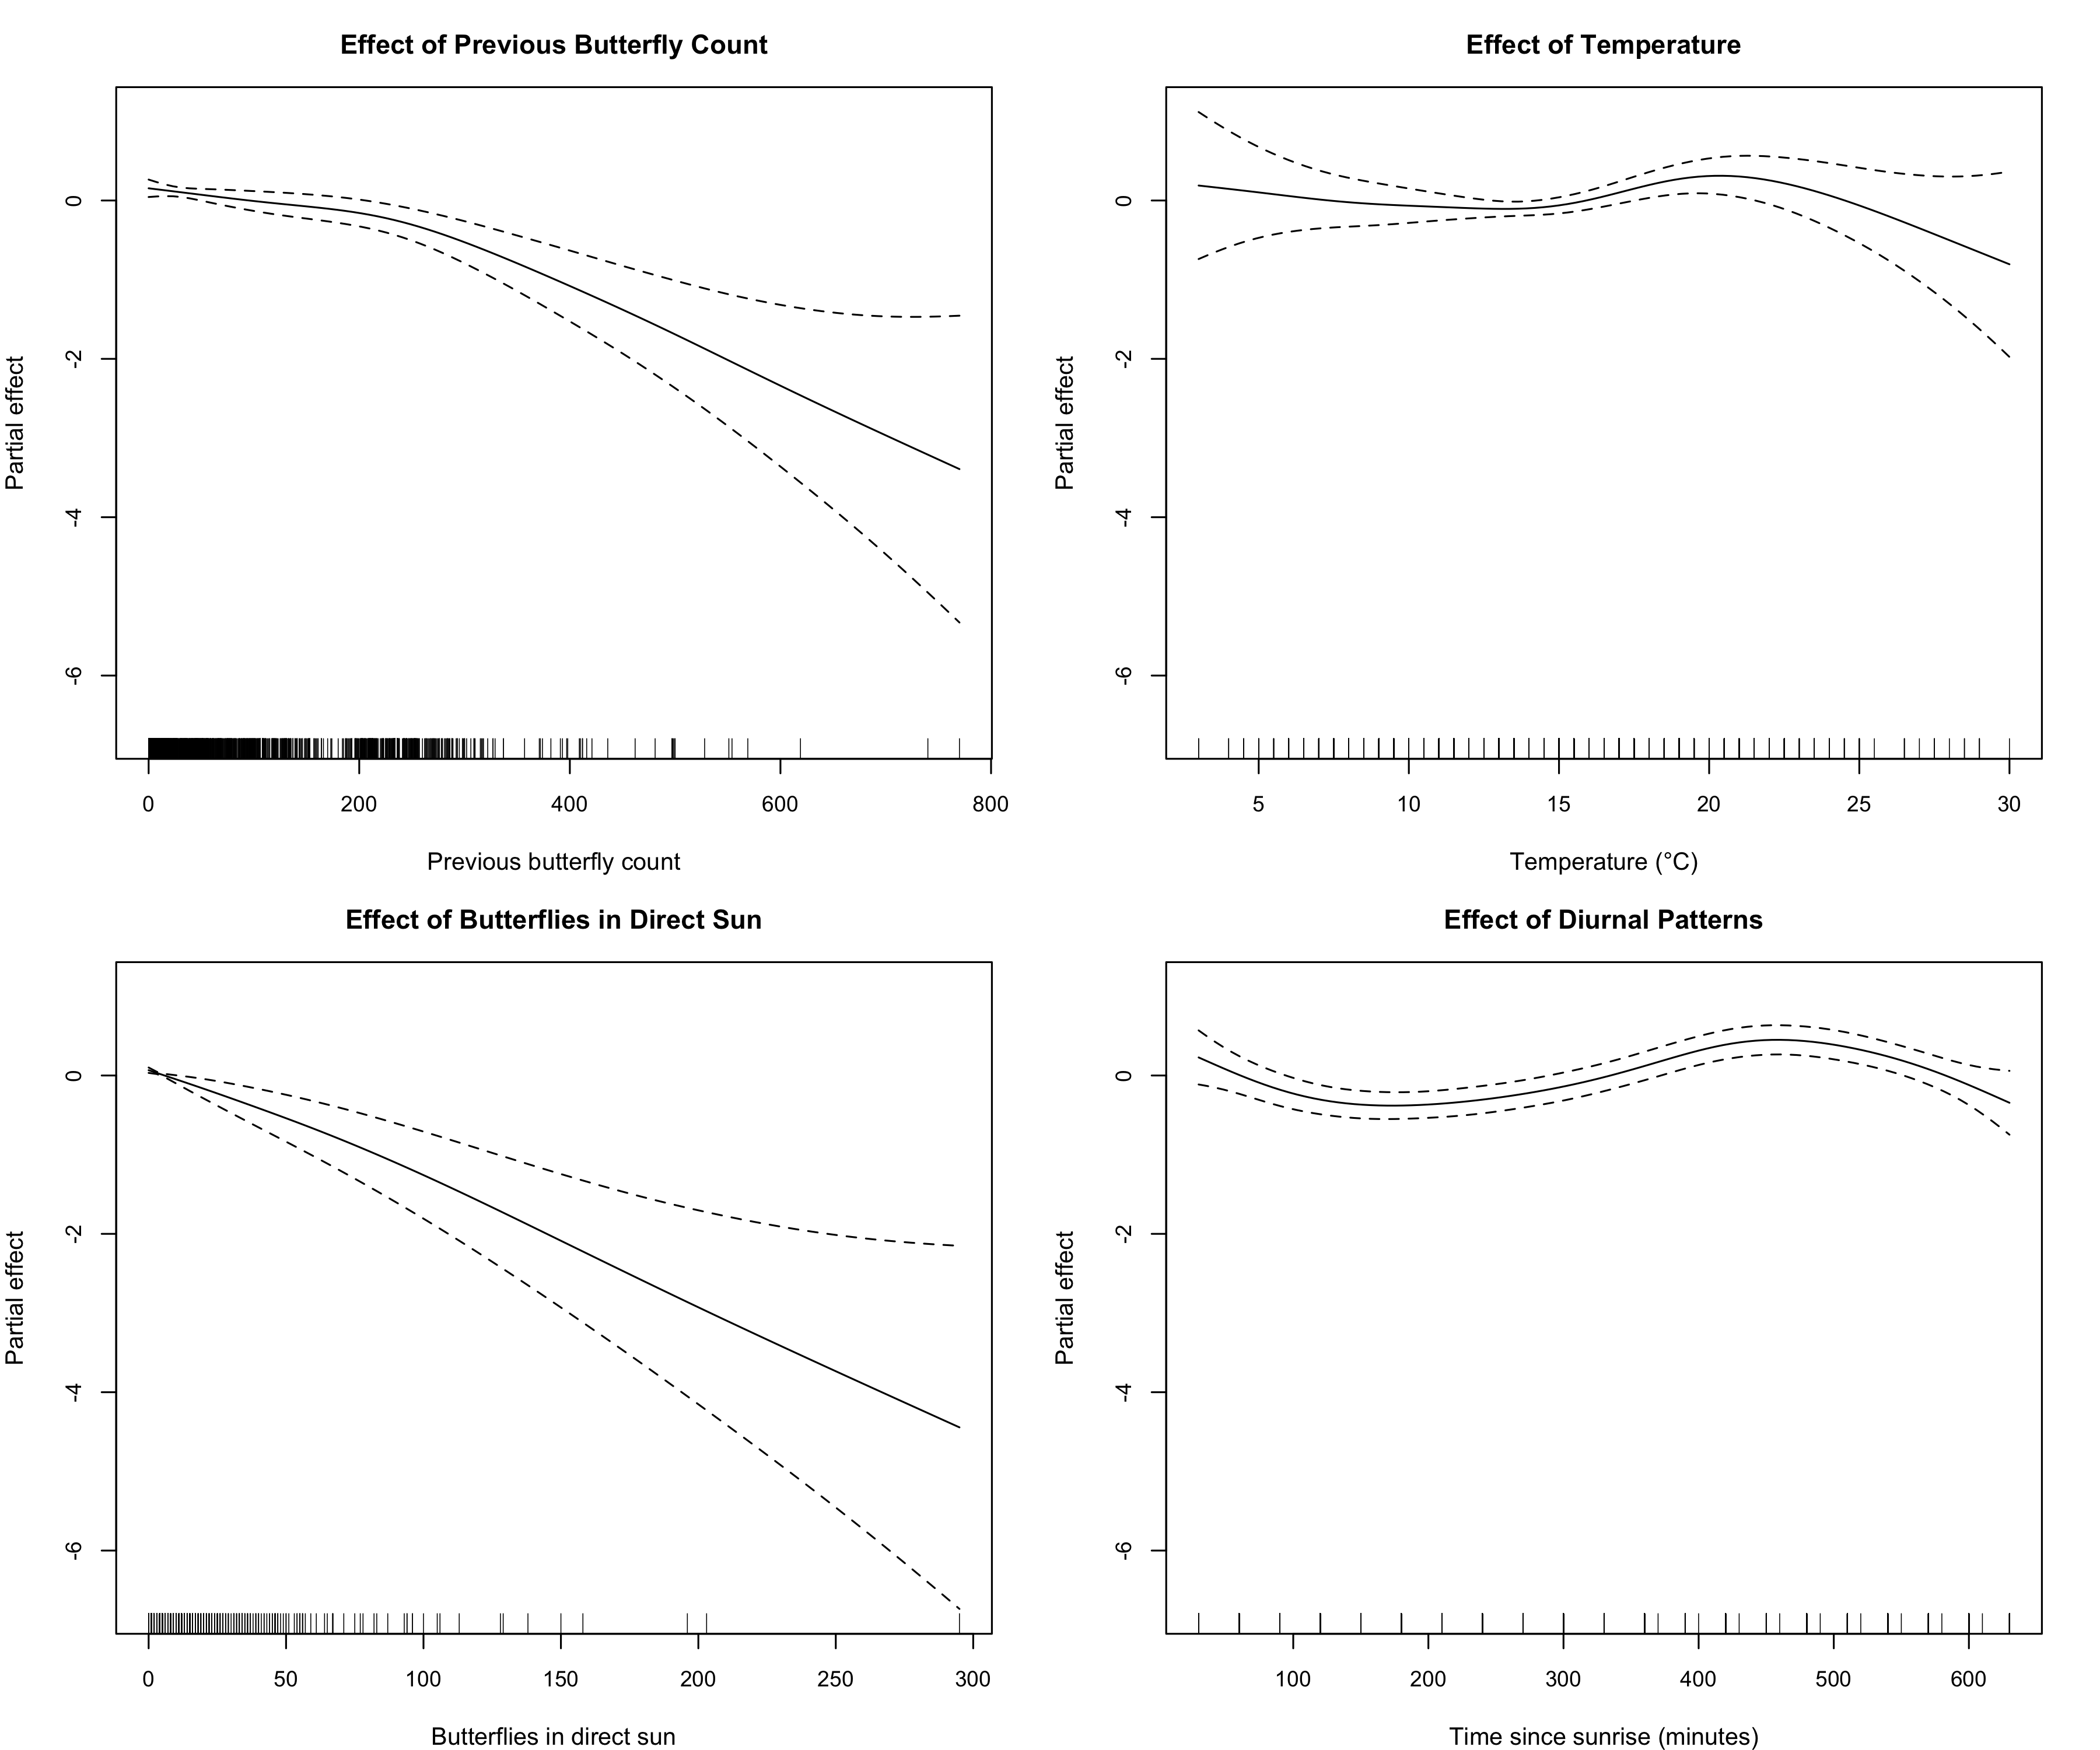
\includegraphics[width=\textwidth]{supplemental/results/thesis_exports/figures/combined_partial_effects.png}
  \caption{Partial effect plots for predictors in the best-fit GAM: lagged roost size, average temperature, direct sun exposure, and time within day. Shaded areas indicate 95\% confidence intervals.}
  \label{fig:partial_effects}
\end{figure}

\subsection{Evaluation of the Disruptive Wind Hypothesis}

We evaluated three hierarchical hypotheses about wind effects on overwintering monarchs:

- Hypothesis 1 (wind as a disruptive force): Not supported. Wind predictors did not appear in the top-performing models under AIC-based selection, indicating wind was not a primary driver of short-interval changes in roost abundance.
- Hypothesis 2 (disruption above a 2\,m/s threshold): Not supported. A sensitivity analysis using a threshold variable (minutes with wind speed \(>\) 2\,m/s) also failed to yield models with improved support.
- Hypothesis 3 (disruption scaling with intensity): Not supported. The gust intensity predictor (\texttt{max\_gust}) did not appear in top-ranked models.

The two wind metrics used in these parallel tests (\texttt{max\_gust} and minutes above threshold) were themselves highly correlated (\(r = 0.78\)), suggesting they capture similar aspects of the wind regime without explaining changes in roost abundance.

\begin{figure}[H]
  \centering
  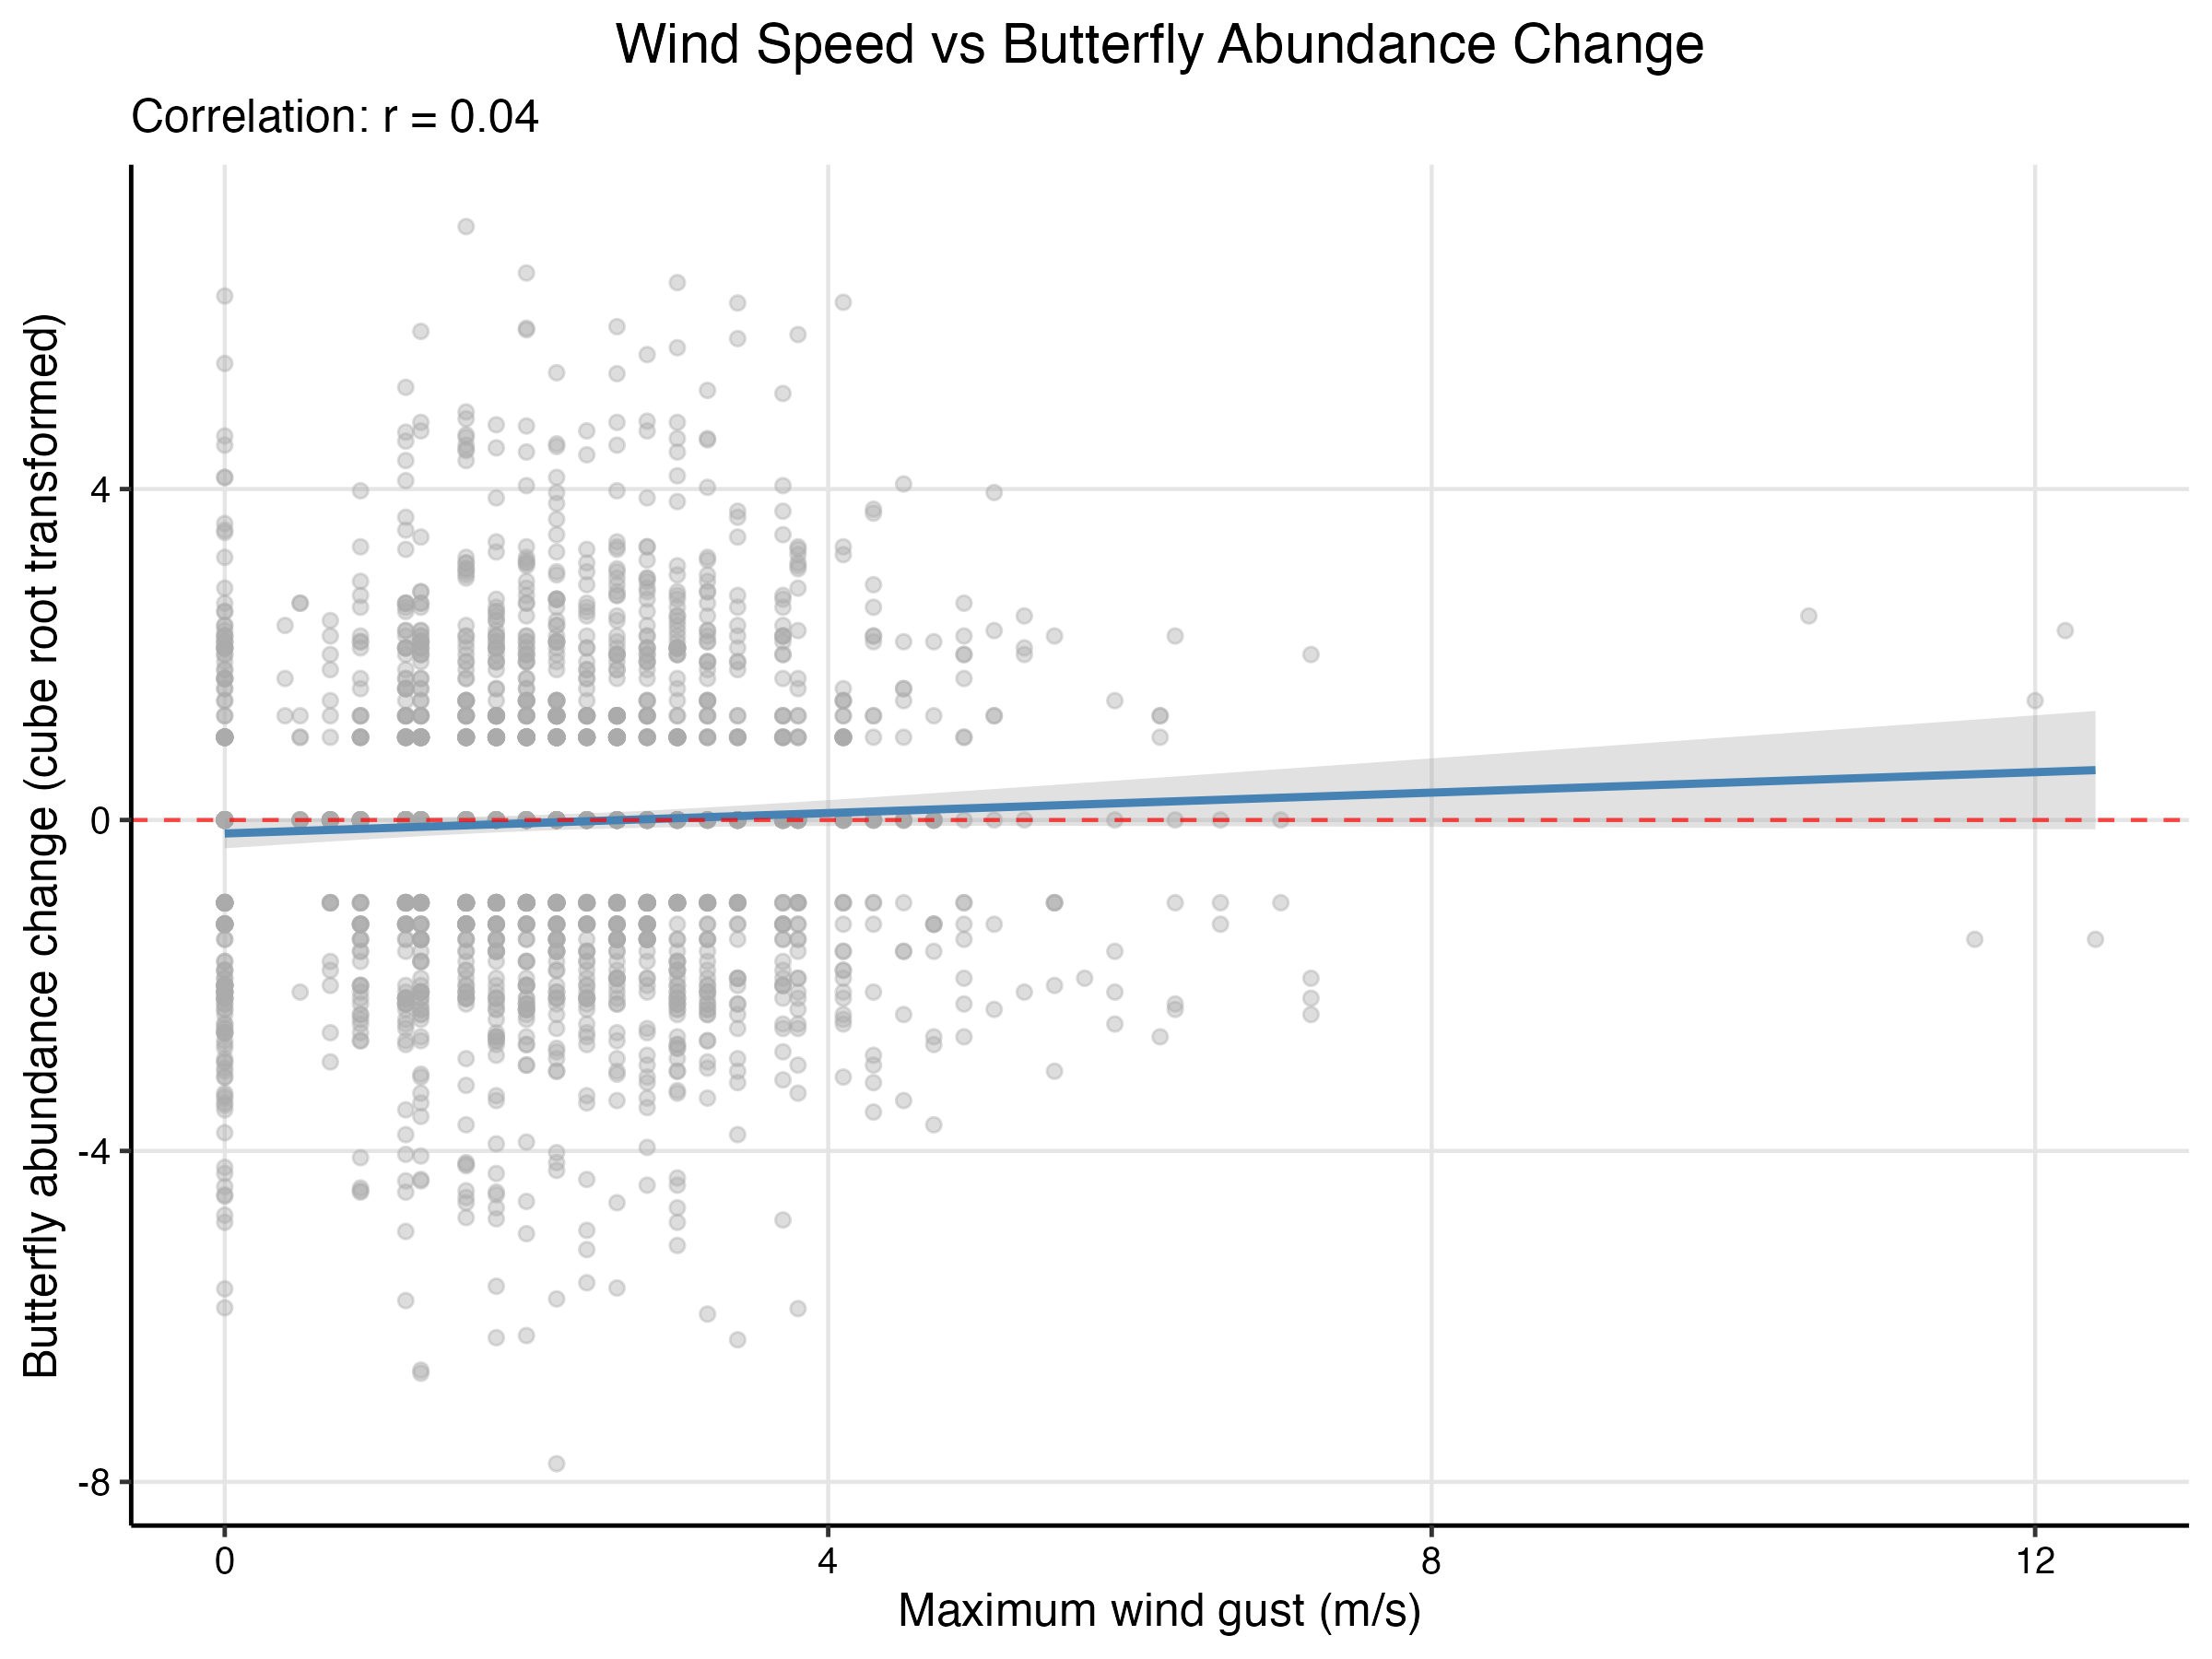
\includegraphics[width=0.8\textwidth]{supplemental/results/thesis_exports/figures/wind_hypothesis_scatter.png}
  \caption{Relationship between gust intensity (\texttt{max\_gust}) and cube-root transformed change in roost abundance. The fitted trend line is approximately flat with confidence intervals overlapping zero across the observed range, consistent with a lack of association.}
  \label{fig:wind_scatter}
\end{figure}


\subsection{Model Diagnostics}

Model diagnostics were consistent with the above findings while revealing limitations inherent to the response structure:

- Residuals vs. fitted: Residuals exhibited visible linear banding/patterning, indicative of unexplained structure arising from the discretized, binned counting method underlying the response (Figure~\ref{subfig:resid_fitted}).
- Normal Q–Q: Residuals were approximately normal with some tail deviations, consistent with the structure observed in the residuals–fitted plot (Figure~\ref{subfig:qq}).

\begin{figure}[H]
  \centering
  \begin{subfigure}[b]{0.58\textwidth}
    \centering
    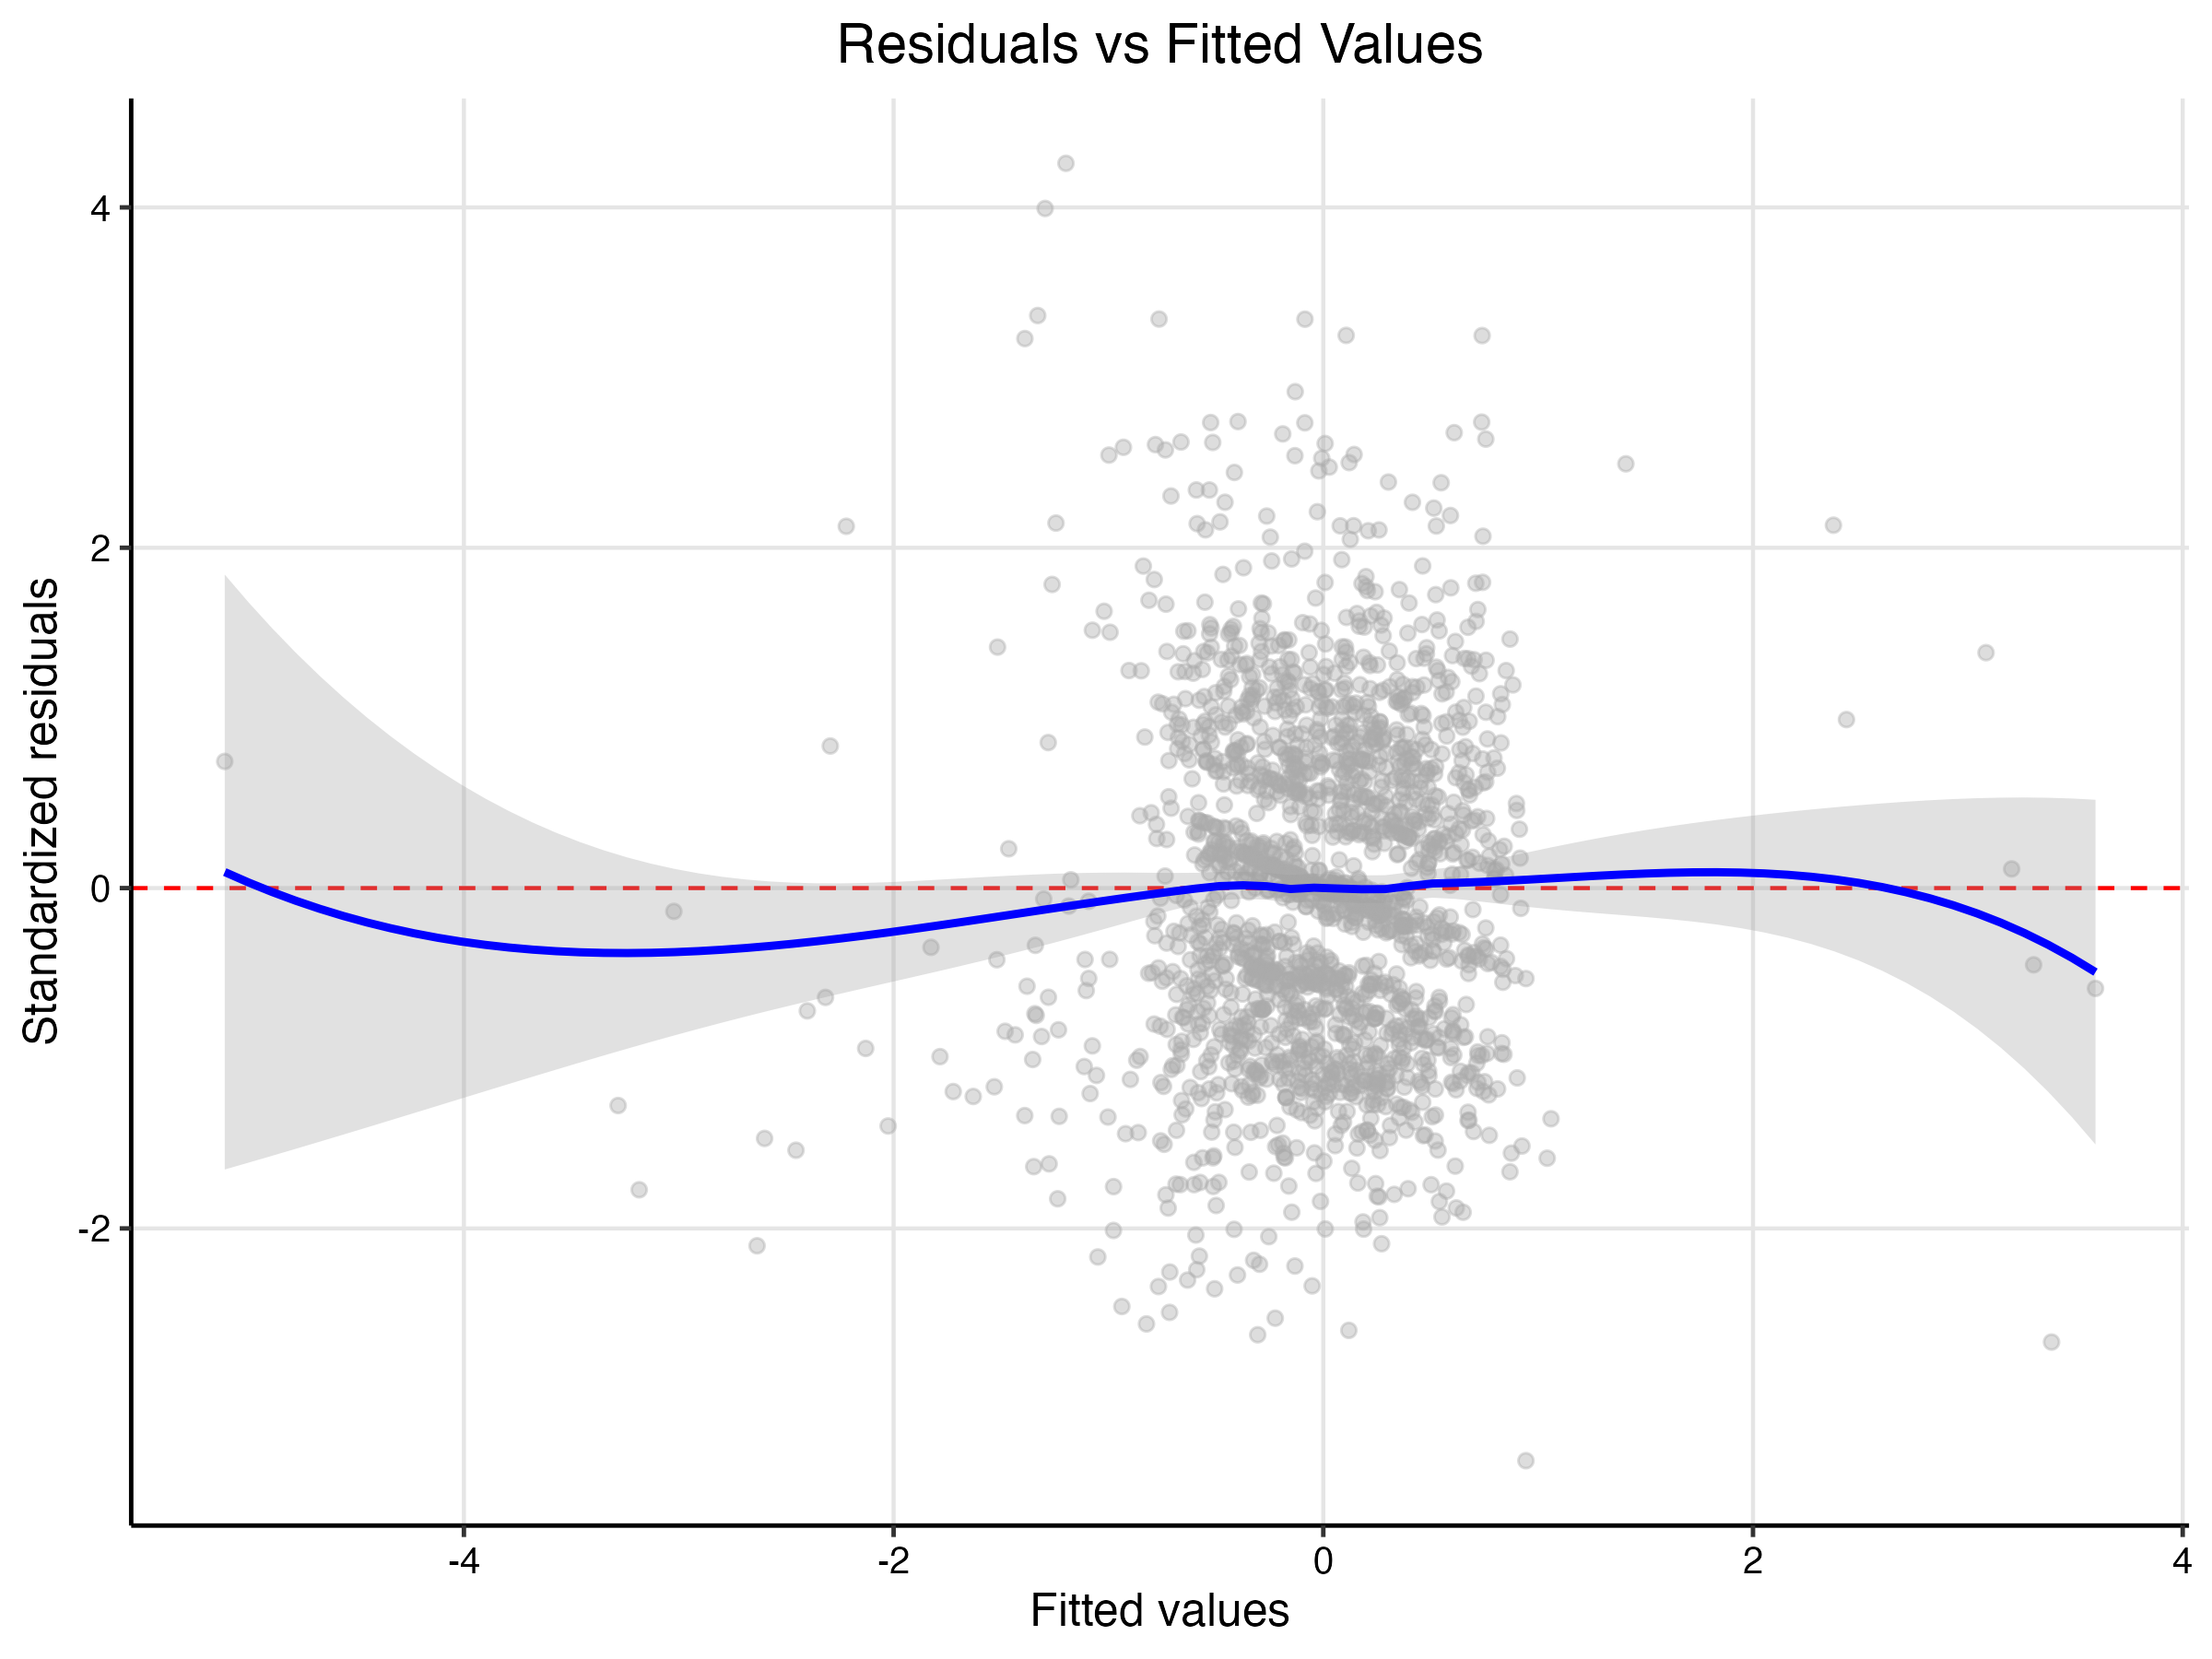
\includegraphics[width=\textwidth]{supplemental/results/thesis_exports/figures/residuals_vs_fitted.png}
    \caption{Residuals vs. fitted}
    \label{subfig:resid_fitted}
  \end{subfigure}\hfill
  \begin{subfigure}[b]{0.38\textwidth}
    \centering
    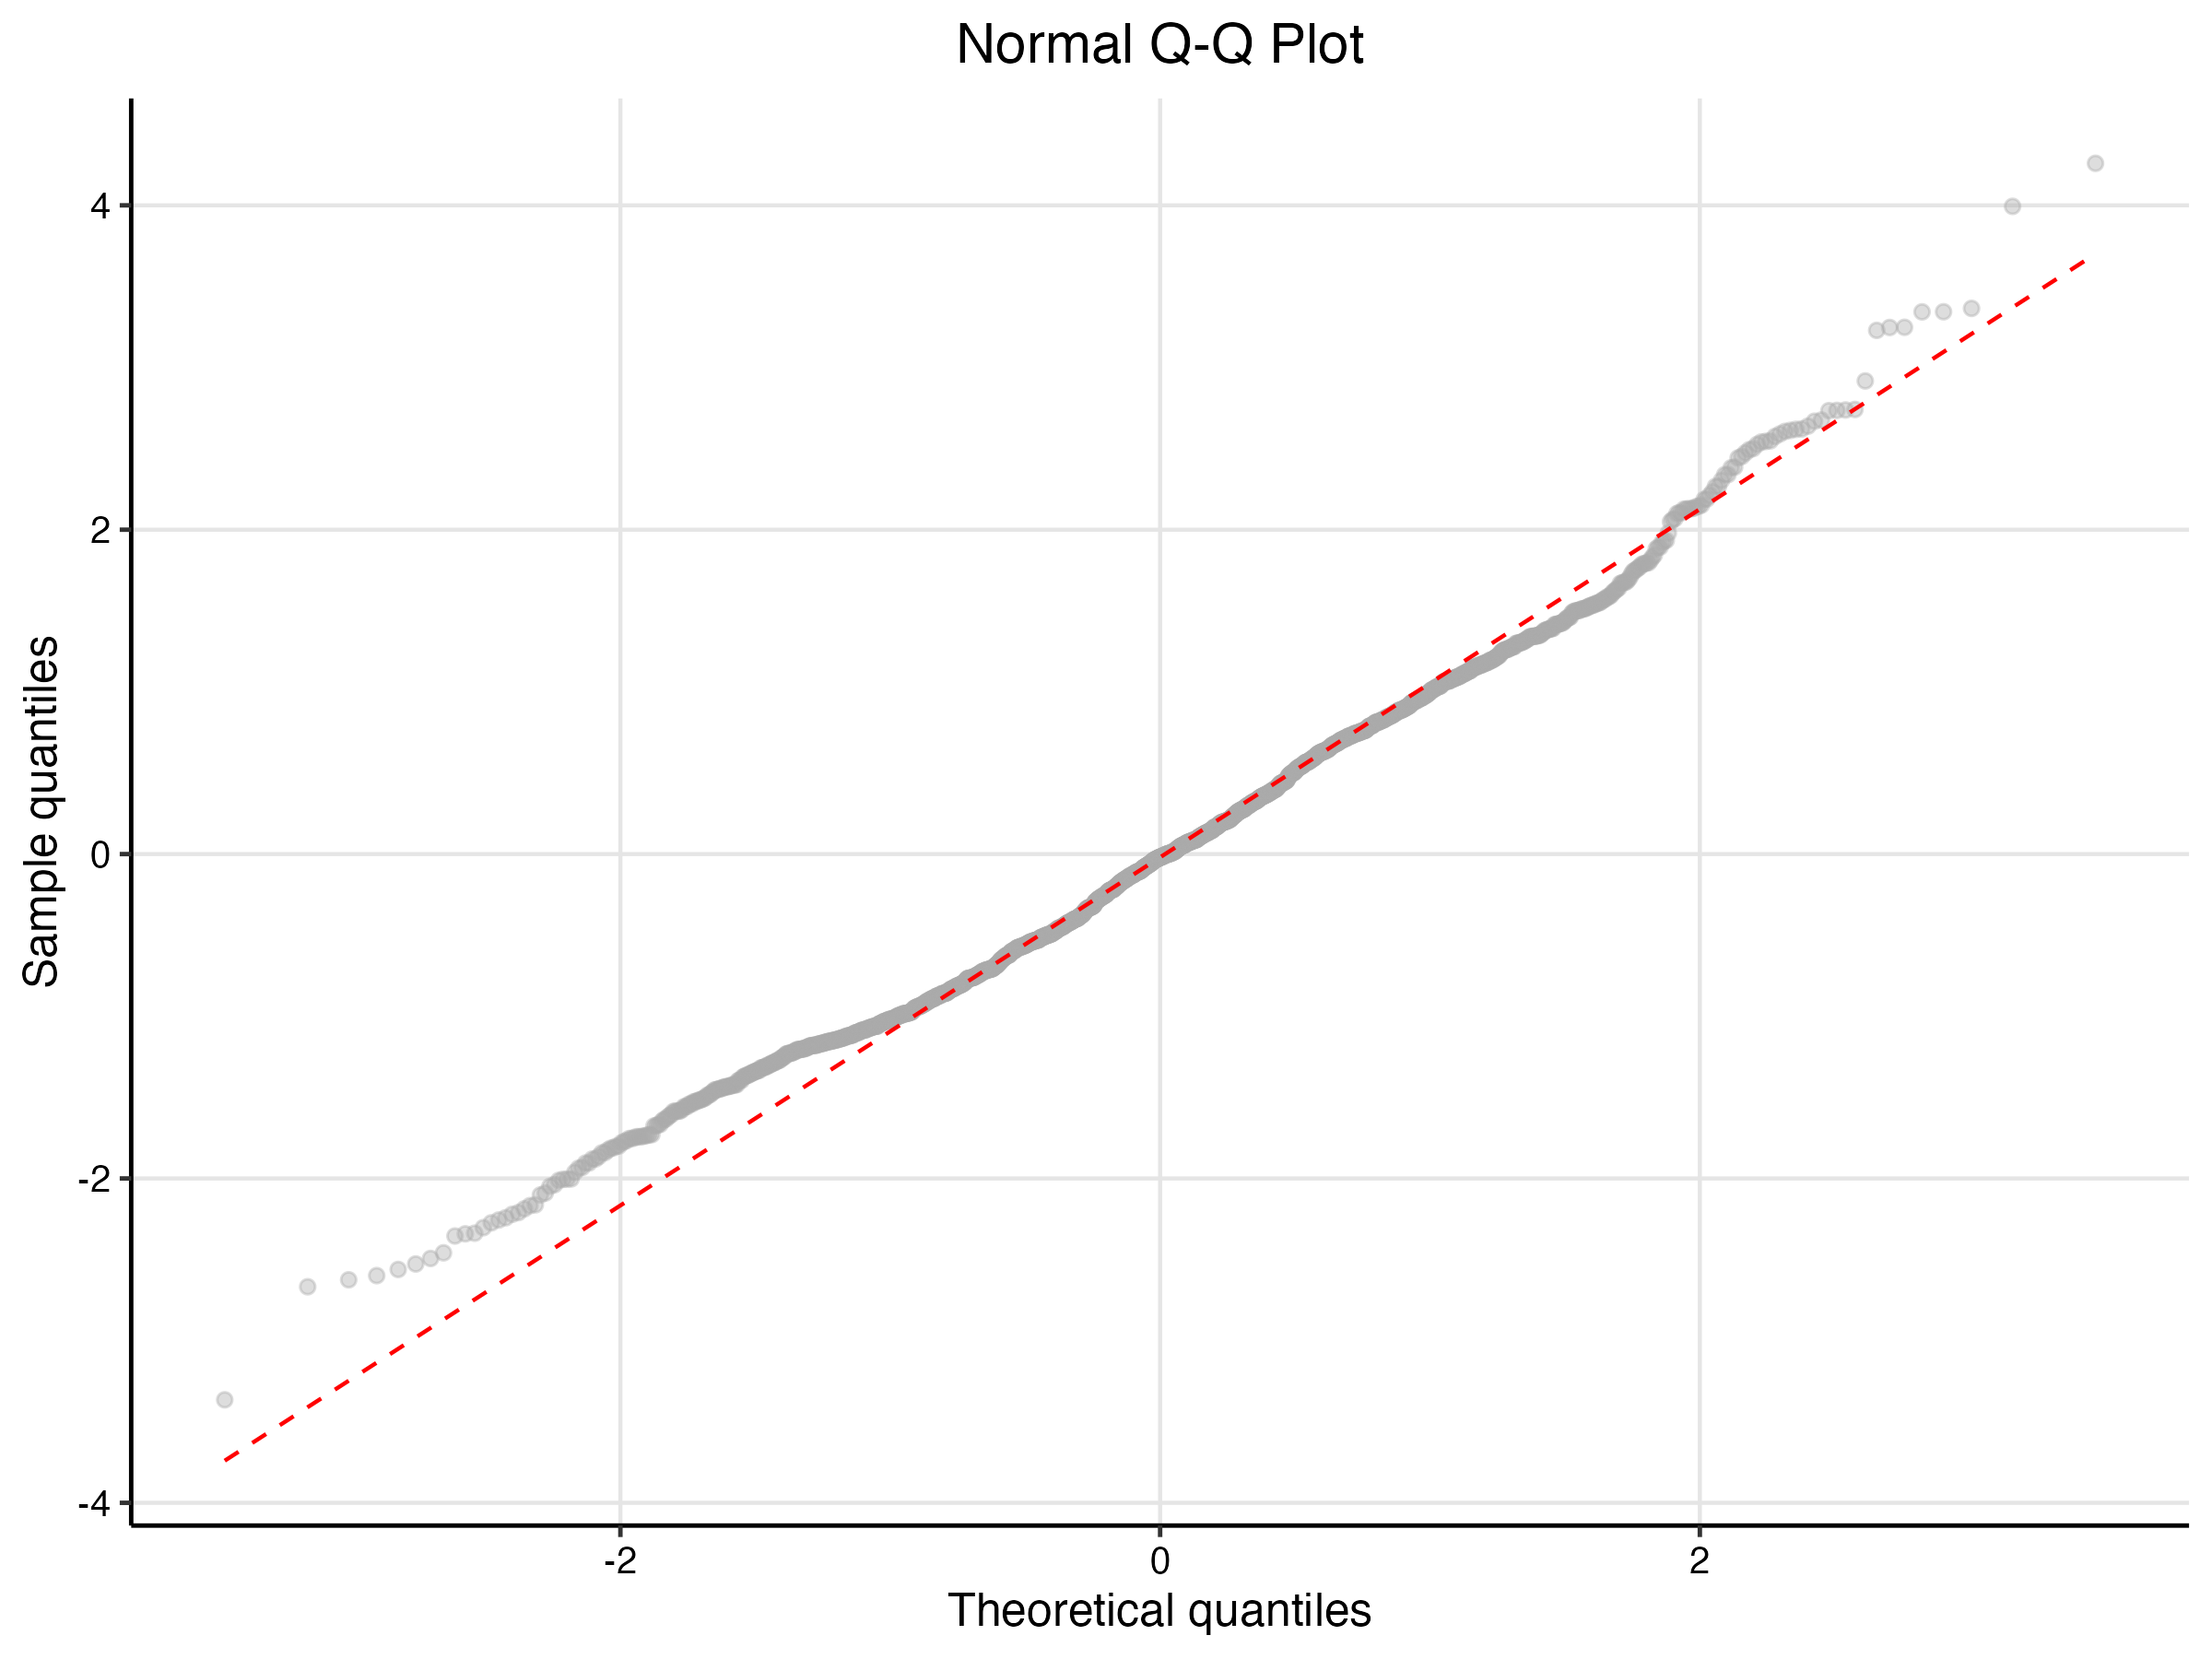
\includegraphics[width=\textwidth]{supplemental/results/thesis_exports/figures/qq_plot.png}
    \caption{Normal Q–Q}
    \label{subfig:qq}
  \end{subfigure}
  \caption{Model diagnostic plots for the best-fit GAM.}
  \label{fig:diagnostics}
  \end{figure}

% Notes for future revision:
% - Add cross-references (e.g., to model selection table) once labels are set in exported tables if desired.
